\documentclass{beamer}
\usepackage{ctex, hyperref}
\usepackage[T1]{fontenc}
% \usepackage[orientation=landscape,size=custom,width=16,height=9,scale=0.4,debug]{beamerposter}
% 修改 slides 比例,

% other packages
\usepackage{latexsym,amsmath,xcolor,multicol,booktabs,calligra}
\usepackage{graphicx,pstricks,listings,stackengine,cite, multirow}
\usepackage{algorithm,algpseudocode,amsmath}    % 写伪代码需要的包
\renewcommand{\algorithmicrequire}{\textbf{Input:}}  % Use Input in the format of Algorithm
\renewcommand{\algorithmicensure}{\textbf{Output:}} % Use Output in the format of Algorithm

\setbeamertemplate{bibliography item}[text]
% \bibliographystyle{plain}
% 如果参考文献太多的话,可以像下面这样调整字体:
\tiny\bibliographystyle{plain}

\author[张三]{学~~~~~~生:张~~~~~三~~~~~~~~\vskip 5pt 指导教师:张~三~三~教授}
\title{基于xxxxx的研究与实现}
\subtitle{~~~~~~~~~~~~~~~~——毕业设计开题答辩}
\institute[哈尔滨工业大学~计算机科学与技术学院]{\small \vskip 45pt哈尔滨工业大学~计算机科学与技术学院}
\date{\small \vskip -17pt二〇二一年六月}
\usepackage{College}

% defs
\def\cmd#1{\texttt{\color{red}\footnotesize $\backslash$#1}}
\def\env#1{\texttt{\color{blue}\footnotesize #1}}
\definecolor{deepblue}{rgb}{0,0,0.5}
\definecolor{deepred}{rgb}{0.6,0,0}
\definecolor{deepgreen}{rgb}{0,0.5,0}
\definecolor{halfgray}{gray}{0.55}

\lstset{
    basicstyle=\ttfamily\small,
    keywordstyle=\bfseries\color{deepblue},
    emphstyle=\ttfamily\color{deepred},    % Custom highlighting style
    stringstyle=\color{deepgreen},
    numbers=left,
    numberstyle=\small\color{halfgray},
    rulesepcolor=\color{red!20!green!20!blue!20},
    frame=shadowbox,
}


\begin{document}

\kaishu
\begin{frame}
    \vspace{-15mm}
    \titlepage
    \vspace{-43mm}
    \begin{figure}[htbp]
      \begin{center}
        
\includegraphics[width=0.16\linewidth]{pic/hit.jpeg}
      \end{center}
    \end{figure}
\end{frame}

\begin{frame}
    \tableofcontents[sectionstyle=show,subsectionstyle=show/shaded/hide,subsubsectionstyle=show/shaded/hide]
\end{frame}



\section{研究现状}
% 2
\begin{frame}{研究现状}
    针对JPEG-LS和图像压缩及加密领域,当前研究方向主要集中在:
    \begin{itemize}[<+-| alert@+>] % 当然,除了alert,手动在里面插 \pause 也行
        \item 图像压缩编码方面:JPEG-LS算法本身研究,主要在于提高编码速度和码率控制等方面
        \item 图像加密处理方面:基于混沌系统的图像加密和基于光学变换的图像加密处理
        \item 很少关注于将JPEG-LS压缩编码和加密结合
    \end{itemize}
\end{frame}


\section{研究内容和拟解决问题}

\subsection{研究内容}

\begin{frame}{混沌密码与传统密码学对比}
    \begin{table}[h]
        \centering
        \caption{对比表}
        \begin{tabular}{|l|l|l|}
        \hline
        比较                  & 传统密码学      & 混沌系统        \\ \hline
        \multirow{3}{*}{相同} & 密钥敏感       & 对初始值敏感      \\ \cline{2-3} 
                            & 扩散         & 混沌运动的轨道混合特性 \\ \cline{2-3} 
                            & 混乱         & 混沌迭代序列的伪随机性 \\ \hline
        不同                  & 密钥空间是有限离散集 & 密钥空间是连续实数集  \\ \hline
        \end{tabular}
        
    \end{table}
\end{frame}

\subsection{拟解决问题}

\begin{frame}{排版举例}
    \begin{exampleblock}{无编号公式} % 加 * 
        \begin{equation*}
            J(\theta) = \mathbb{E}_{\pi_\theta}[G_t] = \sum_{s\in\mathcal{S}} d^\pi (s)V^\pi(s)=\sum_{s\in\mathcal{S}} d^\pi(s)\sum_{a\in\mathcal{A}}\pi_\theta(a|s)Q^\pi(s,a)
        \end{equation*}
    \end{exampleblock}
    \begin{exampleblock}{多行多列公式\footnote{如果公式中有文字出现,请用 $\backslash$mathrm\{\} 或者 $\backslash$text\{\} 包含,不然就会变成 $clip$,在公式里看起来比 $\mathrm{clip}$ 丑非常多。}}
        % 使用 & 分隔
        \begin{align}
            Q_\mathrm{target}&=r+\gamma Q^\pi(s^\prime, \pi_\theta(s^\prime)+\epsilon)\\
            \epsilon&\sim\mathrm{clip}(\mathcal{N}(0, \sigma), -c, c)\nonumber
        \end{align}
    \end{exampleblock}
\end{frame}

\begin{frame}
    \begin{exampleblock}{编号多行公式}
        % Taken from Mathmode.tex
        \begin{multline}
            A=\lim_{n\rightarrow\infty}\Delta x\left(a^{2}+\left(a^{2}+2a\Delta x+\left(\Delta x\right)^{2}\right)\right.\label{eq:reset}\\
            +\left(a^{2}+2\cdot2a\Delta x+2^{2}\left(\Delta x\right)^{2}\right)\\
            +\left(a^{2}+2\cdot3a\Delta x+3^{2}\left(\Delta x\right)^{2}\right)\\
            +\ldots\\
            \left.+\left(a^{2}+2\cdot(n-1)a\Delta x+(n-1)^{2}\left(\Delta x\right)^{2}\right)\right)\\
            =\frac{1}{3}\left(b^{3}-a^{3}\right)
        \end{multline}
    \end{exampleblock}
\end{frame}

\begin{frame}{图形与分栏}
    % From thuthesis user guide.
    \begin{minipage}[c]{0.3\linewidth}
        \psset{unit=0.8cm}
        \begin{pspicture}(-1.75,-3)(3.25,4)
            \psline[linewidth=0.25pt](0,0)(0,4)
            \rput[tl]{0}(0.2,2){$\vec e_z$}
            \rput[tr]{0}(-0.9,1.4){$\vec e$}
            \rput[tl]{0}(2.8,-1.1){$\vec C_{ptm{ext}}$}
            \rput[br]{0}(-0.3,2.1){$\theta$}
            \rput{25}(0,0){%
            \psframe[fillstyle=solid,fillcolor=lightgray,linewidth=.8pt](-0.1,-3.2)(0.1,0)}
            \rput{25}(0,0){%
            \psellipse[fillstyle=solid,fillcolor=yellow,linewidth=3pt](0,0)(1.5,0.5)}
            \rput{25}(0,0){%
            \psframe[fillstyle=solid,fillcolor=lightgray,linewidth=.8pt](-0.1,0)(0.1,3.2)}
            \rput{25}(0,0){\psline[linecolor=red,linewidth=1.5pt]{->}(0,0)(0.,2)}
%           \psRotation{0}(0,3.5){$\dot\phi$}
%           \psRotation{25}(-1.2,2.6){$\dot\psi$}
            \psline[linecolor=red,linewidth=1.25pt]{->}(0,0)(0,2)
            \psline[linecolor=red,linewidth=1.25pt]{->}(0,0)(3,-1)
            \psline[linecolor=red,linewidth=1.25pt]{->}(0,0)(2.85,-0.95)
            \psarc{->}{2.1}{90}{112.5}
            \rput[bl](.1,.01){C}
        \end{pspicture}
    \end{minipage}\hspace{1cm}
    \begin{minipage}{0.5\linewidth}
        \medskip
        %\hspace{2cm}
        \begin{figure}[h]
            \centering
            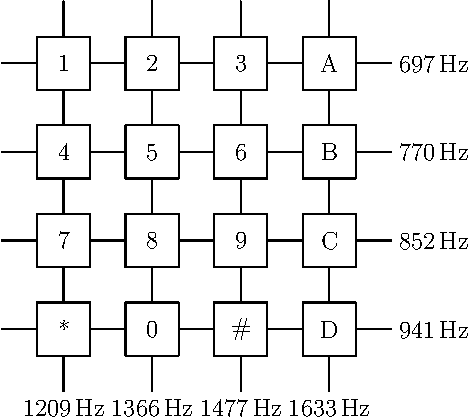
\includegraphics[height=.4\textheight]{pic/dtmf.pdf}
        \end{figure}
    \end{minipage}
\end{frame}

\section{技术路线}

\begin{frame}{算法}
    \begin{algorithm}[H]  
        \caption{Conjugate Gradient Algorithm with Dynamic Step-Size Control}  
        \label{alg::conjugateGradient}  
        \begin{algorithmic}[1]  
          \Require  
            $f(x)$: objective funtion;  
            $x_0$: initial solution;  
            $s$: step size;  
          \Ensure  
            optimal $x^{*}$  
          \State initial $g_0=0$ and $d_0=0$;  
          \Repeat  
            \State compute gradient directions $g_k=\bigtriangledown f(x_k)$;  
            \State compute Polak-Ribiere parameter $\beta_k=\frac{g_k^{T}(g_k-g_{k-1})}{\parallel g_{k-1} \parallel^{2}}$;  
            \State compute the conjugate directions $d_k=-g_k+\beta_k d_{k-1}$;  
            \State compute the step size $\alpha_k=s/\parallel d_k \parallel_{2}$;  
          \Until{($f(x_k)>f(x_{k-1})$)}  
        \end{algorithmic}  
      \end{algorithm}  
\end{frame}

\section{计划安排}

\begin{frame}
    \begin{table}[h]
        \centering
        \caption{ 进度安排}
        \begin{tabular}{|l|l|l|}
        \hline
        阶段   & 时间            & 进度                                                                                 \\ \hline
        第一阶段 & 2021.1-2021.2 & \begin{tabular}[c]{@{}l@{}}确定毕业设计课题,撰写开题报告\\ 并寻找相关资料,了解课题\end{tabular}             \\ \hline
        第二阶段 & 2021.2-2021.3 & \begin{tabular}[c]{@{}l@{}}学习JPEG-LS算法,并进行相关实践,\\ 尝试加入加密功能,形成初步的整体思路。\end{tabular} \\ \hline
        第三阶段 & 2021.4        & 准备毕业设计中期答辩                                                                         \\ \hline
        第四阶段 & 2021.4-2021.5 & 逐步完成算法理论研究,进行系统实现                                                                \\ \hline
        第五阶段 & 2021.5-2021.6 & 完成毕业设计论文,准备毕业设计答辩                                                                  \\ \hline
        \end{tabular}
    \end{table}
\end{frame}

\begin{frame}
    \begin{center}
        感谢各位老师的聆听!    
    \end{center}
\end{frame}

\section{参考文献}

\begin{frame}[allowframebreaks]
    \nocite{*}
    \bibliography{ref}
\end{frame}


\end{document}
